\section{Low-Power Modes \refskript{7.3.6}}
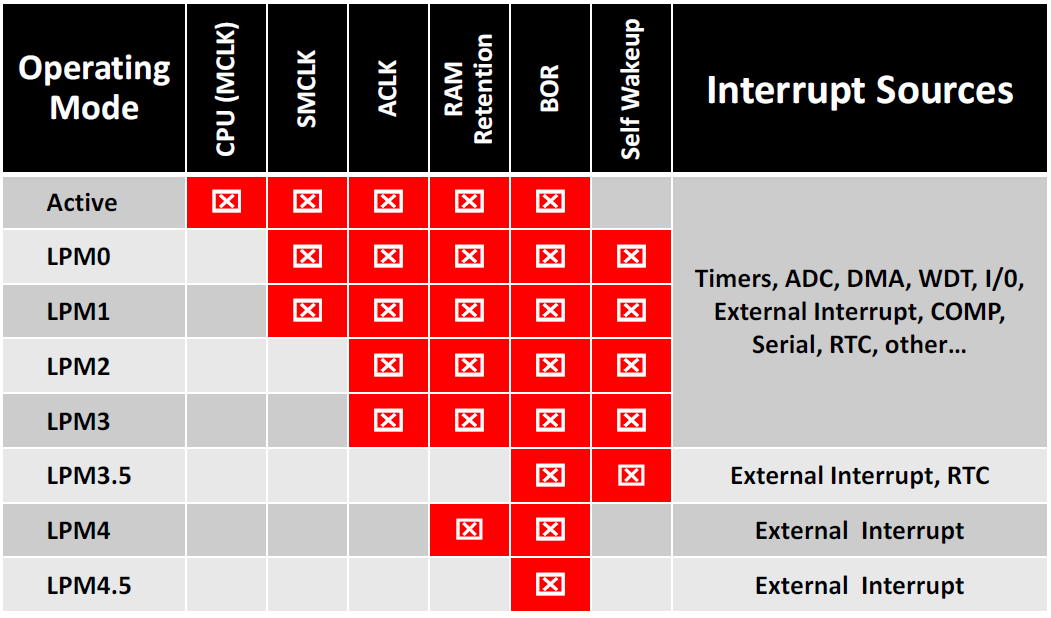
\includegraphics[width=.8\columnwidth, center]{Images/LPO_interrupts.png}

\subsection{Activity Profiles}

\subsection{Power Consumption in CMOS Technology}
\begin{minipage}{0.5\columnwidth}
	\vspace{0pt}
	\formula{$P \sim \alpha C_L V_{dd}^2 f$}
	\formula{$E \sim  \alpha C_L V_{dd}^2 f t$}
	\formula{$E \sim \alpha C_L V_{dd}^2 \mathit{(\# cycles)}$}
	
	\formula{$\tau \sim C_L \dfrac{V_dd}{(V_dd - V_T)^2}$}
	\formula{$f \sim \dfrac{1}{\tau} \sim V_{dd}$}
\end{minipage}
\begin{minipage}{0.5\columnwidth}
	\vspace{0pt}
	\unitText{$V_{dd}$}{supply voltage}{\unit{V}}\\
	\unitText{$V_T$}{threshold voltage}{\unit{V}}
	\unitText{$\alpha$}{switching activity}{\unit{1}}\\
	\unitText{$C_L$}{load capacity}{\unit{F}}\\
	\unitText{$f$}{clock frequency}{\unit{Hz}}\\
	\unitText{$\tau$}{Gate delay}{\unit{ms}}
\end{minipage}
\vspace{2mm}


\subsection{Interrupts and Low-Power Modes}
Low power modes are configured with the bits \textit{CPUOFF}, \textit{OSCOFF}, \textit{SCG0} and \textit{SCG1} in the \textbf{Status Register} (SR, also called R2).

\subsection{CCS6 Intrinsic Functions for MSP430}
\begin{lstlisting}[language=c]
	#include <intrinsics.h>
\end{lstlisting}

\subsection{Low-Power Optimization}
Replace software with hardware peripherals.
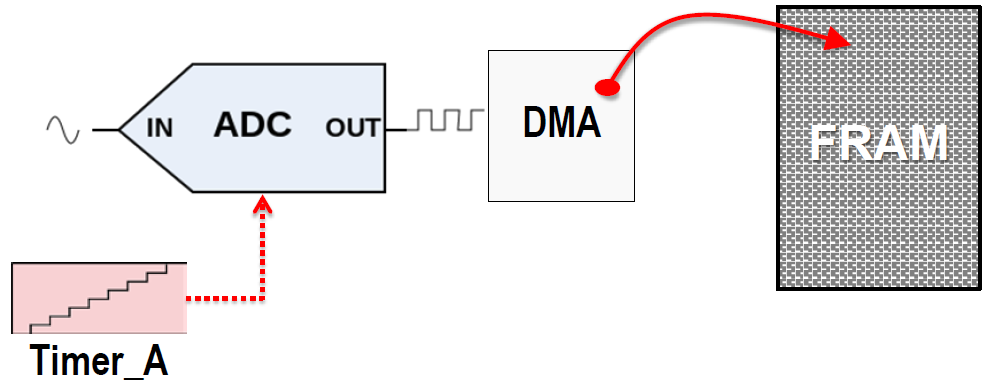
\includegraphics[width=0.8\columnwidth, center]{Images/LPM_replace_hw_with_sw.png}

\section{Real-Time Clock (RTC) \refskript{7.4.3}}
\subsection{RTC Interrupts}
\begin{enumerate}
	\itemsep-.5em 
	\item Alarm
	\item Interval Timer
	\item Prescaler 0
	\item Prescaler 1
	\item Ready for Register operation
\end{enumerate}

Example 1: Time Event
\begin{lstlisting}[language=C]
int main (void)
{
	WDTCTL = WDTPW | WDTHOLD;	//stop watchdog
	//disable high-impedance ports
	PM5CTL0 &= ~LOCKLPM5;
	//just for testing (P1.0 / LED1)
	P1DIR |= 0x01;
	P1OUT &= ~0x01;
	
	PJSEL0 = BIT4 | BIT5; //Init. LFXT pins
		
	//Configure LFXT 32kHz crystal
	CSCTL0_H = CSKEY >> 8;	//Unlock CS reg.
	CSCTL4 &= ~LFXTOFF;			//Enable LFXT
	do
	{
		//Clear LFXT fault flag
		CSCTL5 &= ~LFXTOFFG;
		SFRIFG1 &= ~OFIFG;
		//Test oscillator fault flag
	} while (SFRIFG1 & OFIFG);
	CSCTL0_H = 0;	//Lock CS registers
		
	//write RTCKEY to unlock RTC reg. for write
	RTCCTL0_H = 0xA5;
	//hold RTC, clock from output of RT1PS,
	// RTCTEVIFG on 8-bit overflow
	RTCCTL1 = 0x48;
		
	//Enable time event interrupt
	RTCCTL0_L = 0x40;
	//prescale timer 0: divided by 64
	RTCPS0CTL = 0x2800;
	//prescale timer 1: out from RT0PS, div. by 2
	RTCPS1CTL = 0x8000;
	//Enable RTC
	RTCCTL1 &= ~0x40;
	//Enter LPM3 with interrupt enabled
	__bis_SR_register(LPM3_bits + GIE);
		
	while (1)
	{}
}
\end{lstlisting}

Example 2: RTC Calendar
\begin{lstlisting}[language=C]
//BCD, hold RTC, RTCMode, one minute overflow
RTCCTL1 = 0xE0;

RTCSEC = 0x00;	//Set Seconds
RTCMIN = 0x00;	//Set Minutes
RTCHOUR = 0x10;	//Set Hours
RTCDOW = 0x03;	//Set DOW (sunday = 0)
RTCDAY = 0x18;	//Set Day
RTCMON = 0x10;	//Set Month
RTCYEAR = 0x2023;	//Set Year

//setup alarm
//enable minutes alarm, minutes = 1 and others are don't care
// --> so an alarm is generated on 00:01:00, 01:01:00, ...
RTCAMIN = 0x81;
RTCAHOUR = 0x00;
RTCADOW = 0x00;
RTCADAY = 0x01;

RTCCTL0_L = 0x60;
//Enable time event & alarm interrupt
RTCCTL1 &= ~0x40;
//Enable RTC
__bis_SR_register(LPM3_bits + GIE); //Enter LPM3 w/ interrupt
while (1)
{}
\end{lstlisting}




